\subsection{Die Übergangsfunktion}

Die Übergangsfunktion $h(t)$, auch Sprungantwort genannt, ist die Antwort im Zeitbereich auf die Heaviside-Funktion $\sigma(t)$: \[\sigma (t) = \begin{cases} 0 & \text{für t < 0} \\ 1 & \text{für t > 0} \end{cases}\] \newline
In Abbildung \ref{fig:aufbau} ist der Aufbau zu sehen. Das Oszilloskop in Abbildung \ref{fig:oszilloskop} zeigt die Sprungantwort im Simulationsintervall 0 - 100 an. \newline
In Abbildung \ref{fig:matlab_sprungantwort} ist die Übergangsfunktion in Matlab vom Intervall 0 bis 3500 zu sehen, während Abbildung \ref{fig:matlab100_sprungantwort} die Sprungantwort im Intervall 0 bis 100 zeigt. \\
Die Steigung der Asymptoten der Sprungantwort entspricht dem statischen Verstärkungsfaktor $K=4$.

\begin{figure}[H]
	\centering
	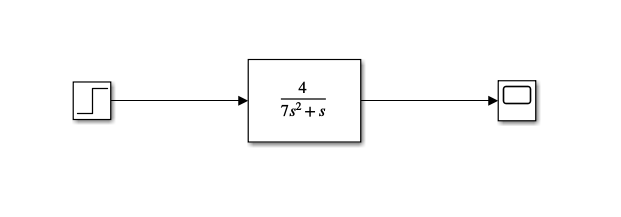
\includegraphics[width=0.8\textwidth]{{diagrams/aufbau.png}}
	\caption[Aufbau]{Aufbau in Simulink}
	\label{fig:aufbau}
\end{figure}

\begin{figure}[H]
	\centering
	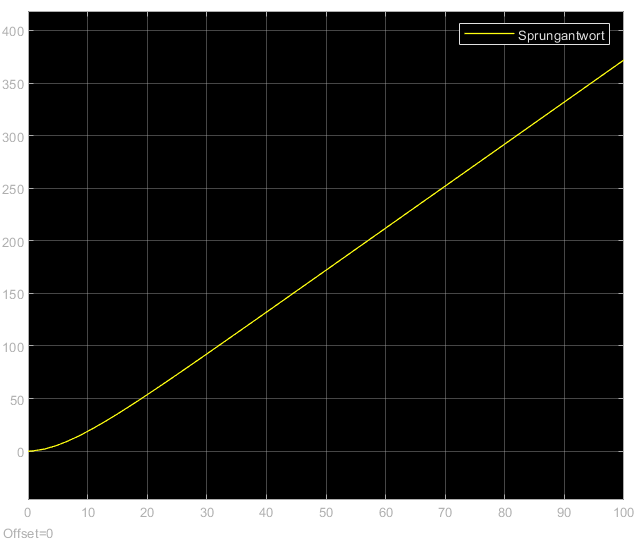
\includegraphics[width=0.8\textwidth]{{diagrams/sprungantwort_simulink_100.png}}
	\caption[Oszilloskop]{Oszilloskop - Sprungantwort im Intervall 0 bis 100}
	\label{fig:oszilloskop}
\end{figure}

\begin{figure}[H]
	\centering
	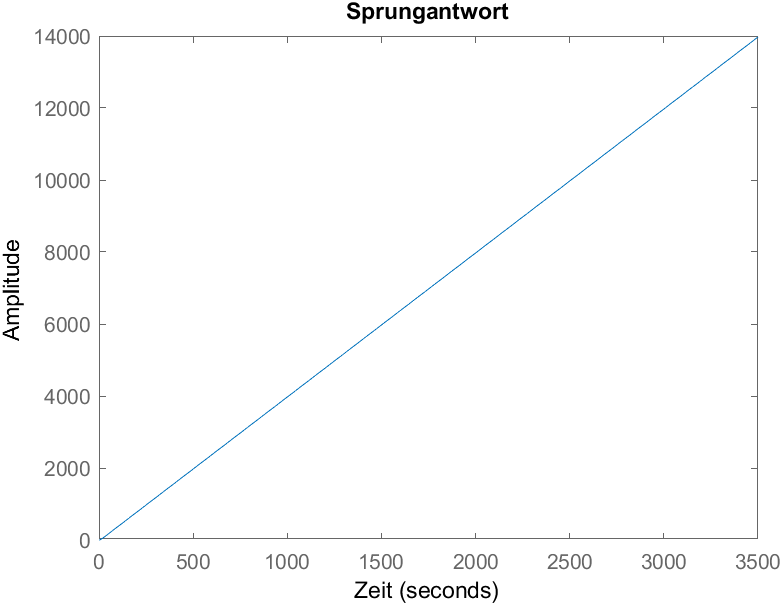
\includegraphics[width=0.8\textwidth]{{diagrams/sprungantwort_matlab.png}}
	\caption[Oszilloskop]{Matlab - Sprungantwort}
	\label{fig:matlab_sprungantwort}
\end{figure}

\begin{figure}[H]
	\centering
	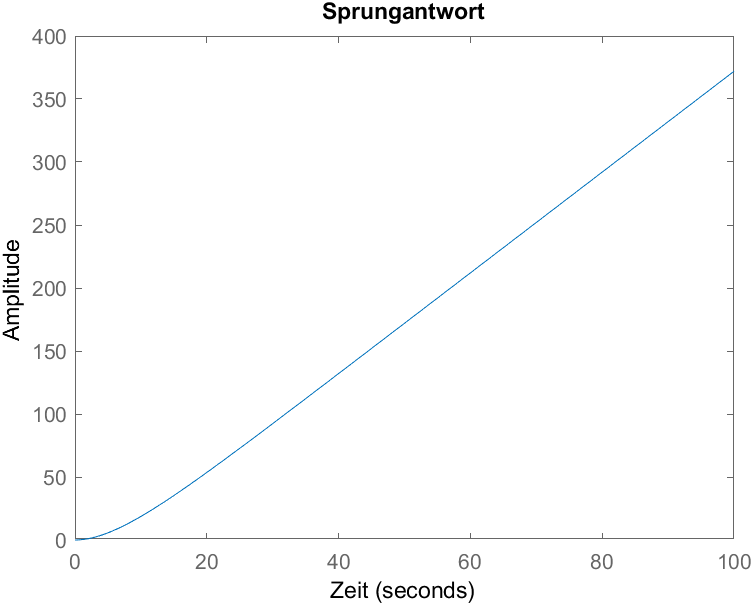
\includegraphics[width=0.8\textwidth]{{diagrams/sprungantwort_matlab_limit100.png}}
	\caption[Oszilloskop]{Matlab - Sprungantwort im Intervall 0 bis 100}
	\label{fig:matlab100_sprungantwort}
\end{figure}